My investigation of the extent and properties of the semantic-pragmatic adaptation processes through the example of adaptation to uncertainty expressions  falls within the broader topic of partner-specific linguistic behavior, which I review in the next section. Since I will also be making use of recent semantic theories of epistemic
modals and game-theoretic pragmatic models, I also provide background on these two topics in this chapter.

\section{Partner-specific linguistic behavior}

Partner-specific linguistic behavior constitutes a large class of behaviors in which language users either change their comprehension behavior or their production behavior or both to better align with the idiosyncrasies of their conversational partners. Both the observed phenomena and the underlying cognitive processes and mechanisms have been discussed under several different names in the literature, including \textit{alignment} \egcite{Pickering2004}, \textit{accommodation} \egcite{Goldinger1998}, \textit{convergence} \egcite{Pardo2006}, \textit{lexical entrainment} \egcite{Clark1986}, and--the topic of this dissertation--\textit{adaptation} \egcite{Kleinschmidt2015}. The multitude of terms stems in part from different scientific communities working on different linguistic domains. For example, the terms \textit{convergence} and \textit{alignment} 
are both generally used to refer to the process of speakers and listeners converging in their production and comprehension behavior in interaction such that after several rounds of interaction, 
their phonetic productions and syntactic preferences are more similar to each other than at the beginning of the interaction. Researchers in phonetics, tend to describe this process as \textit{convergence} 
whereas the sentence processing community prefers the term \textit{alignment}. In part, however, these terms actually describe different phenomena. In particular, research in \textit{adaptation} generally focuses exclusively
on the comprehension side of language processing whereas research on \textit{alignment}, \textit{accommodation}, \textit{convergence}, and \textit{lexical entrainment} generally discusses partner-specific production as well as comprehension behavior, although the focus of most of this research lies on production behavior with the assumption that changes in production behavior follow from changes in comprehension behavior.

Experimental evidence for partner-specific behavior comes mostly from three different forms of studies: \textit{exposure-test} studies, \textit{continuous adaptation} studies, and \textit{interactive conversation} studies.
In exposure-test studies, participants first listen to some linguistic material,  e.g., words in isolation or sentences describing an event depicted on a card.  After this passive exposure, there is generally
some form of test phase that probes whether participants updated their production and/or comprehension behavior. While frequently there is only one exposure and one test phase, there can also be multiple
exposure-test blocks within one experiment.

In continuous adaptation studies, exposure and test trials are combined and thus participants' behavior is probed after each exposure. The behavioral data in these studies often comes from online processing measures such as self-paced reading studies in which participants read a sentence word-by-word and one measures how long it takes them to read each word, or visual-world eye-tracking \cite{Tanenhaus1995} or mouse-tracking \egcite{Roettger2019} in which participants are instructed to point or click on an object and one tracks the movement of their gaze or their cursor.

In interactive conversation studies, either one participant and one confederate or two participants work on a task requiring language. For example, in the director-matcher paradigm, one participant (or a confederate) takes the role of the director who describes the order of different pictures in a display in front of them that is occluded from the other participant's vision, and the other participant (the matcher) has to put the same set of pictures into the same order 
as the director's set of pictures. The dependent measure in these experiments are usually either the recordings or transcripts which can be analyzed in terms of how similar the production behavior of the two interlocutors becomes over time, or one can also employ online measures such as eye-tracking to draw inferences about the comprehension behavior of the matcher.

Such experiments have been used in hundreds, if not thousands, of studies to investigate partner-specific linguistic behavior. I will not be able to review all of them or even the majority of them, but in what follows, I will present several foundational studies across linguistic domains and then discuss theories and computational models of partner-specific behavior. Finally, I will discuss several of the core questions regarding partner-specific behavior and what different accounts predict along with results from studies that try to adjudicate between different explanations. 

\subsection{Foundational studies}

\paragraph{Phonetics.} \textcite{Goldinger1998} conducted a series of shadowing experiments to investigate properties of the lexicon. In these exposure-test studies, 
he asked participants to first produce a set of words (or non-words) that were written on a screen (the baseline recordings). Then participants listened to recordings of these stimuli in 
an exposure phase. Finally, participants had to repeat (``shadow'') words in a test phase which were recorded by the experimenter. The main dependent measure
for his experiments came from an AXB task. In an AXB task, participants subsequently listen to three recordings A, X, and B and have to decide whether A sounds more like X
than B does, or B more than A. A and B were always the baseline recording and the shadowing recording (in counterbalanced order) and X was the stimulus token that the shadower had heard
in the shadowing experiment. \textcite{Goldinger1998} found that participants in the AXB task  were consistently more likely to select the shadowing recording than the baseline recording, with modulation
effects from overall word frequency, the number of repetitions of each stimulus, and whether participants immediately shadowed the word or did so after a brief delay. While his main conclusion
from this experiment was that language users store detailed episodes of perceived words in memory, this study was also among the first that provided evidence for phonetic accommodation: 
participants in the shadowing task changed their production behavior such that it matched more closely the behavior of the speaker whose productions they had heard during the exposure phase.

%had a pre-test phase
\textcite{Norris2003} conducted a series of exposure-test phonetic adaptation
experiments investigating whether listeners could shift their perceptual boundaries between phonemes. Their exposure phase
consisted of a lexical decision task; on each trial, Dutch participants listened to a recording and were asked to respond whether
what they heard constituted a Dutch word or not. The recordings varied depending on the condition. In the /f/-biased condition,
participants heard /f?s/, a sound that was ambiguous between the fricatives /f/ and /s/, embedded in words that always end in /f/
in Dutch; and in the /s/-biased condition, participants heard /f?s/ embedded in words that always end in /s/. Thus, the ambiguous sound was always 
disambiguated by the lexical context. During the test phase, participants categorized sounds on a continuum from /f/ to /s/ as either /f/ or /s/. \textcite{Norris2003}
found that participants in the /f/-biased condition categorized more sounds on the continuum as /f/ than participants in the /s/-biased condition,
suggesting that listeners shifted their perceptual boundary in response to the speech in the exposure phase.
 
 \textcite{Clayards2008} studied another aspect of adaptation, namely whether listeners also update their beliefs about the intra-speaker variability
 of phonetic features. Specifically, they looked at the variance in voice-onset times (VOT) of the bilabial stops /p/ and /b/. Subjects participated in a visual-world
 eye-tracking study in which they saw pictures of four different objects on a screen. On each trial, participants listened to the recording of a single word
 and were asked to click on the object that had been mentioned. On critical trials, there were two objects whose names only differed in the word-initial stop, e.g.,
 a beach and a peach. Across conditions, participants either listened to recordings of a speaker with very consistent VOTs (i.e., the variance in VOTs was very low; \textit{narrow} condition) or
 to a speaker with highly varying VOTs (\textit{wide} condition). \textcite{Clayards2008} found that in the wide condition, participants looked more at the competitor object 
 (e.g., at the beach when hearing \textit{peach}) than in the narrow condition, suggesting that participants exhibited uncertainty about which word the speaker produced
and that over the course of the experiment, they learned the VOT distributions of the speaker.


\paragraph{Syntax.} \textcite{Bock1986} conducted one of the first studies systematically investigating partner-specific syntactic behavior through a repeated
exposure-test experiment. Participants interacted with an experimenter who showed participants cards depicting an event.  Half of the trials were priming trials on which
 participants listened to the experimenter describing the depicted event, and participants were asked to repeat the description of the experimenter. 
 Each priming trial was followed by a picture description trial on which participants were asked to describe a different event depicted on another card without any input from the experimenter.
The critical priming trials varied in terms of the syntactic structure that was used to describe the event. Half of the events could be either described with a prepositional
 prepositional dative construction (e.g., \textit{``A rock star
sold some cocaine to an undercover agent''})  or a double object construction (\textit{``A rock star sold an undercover agent some cocaine''}), and the other half could be
described using an active sentence (e.g., \textit{``One of the fans punched the referee''}) or a passive construction (\textit{``The referee was punched by one of the fans''}).
\cite{Bock1986} found that the syntactic structure descriptions that participants produced on the picture description trials were influenced by the syntactic structure of the description
of the priming trial; for example, when participants described an event after hearing a prepositional dative description on the preceding priming trial, they were more likely to also 
use a prepositional dative description than when they were primed with a double object construction. These findings, usually referred to as syntactic priming, have been 
replicated many times, including in interactive conversations between two participants \cite{Branigan2000} and in comprehension \egcite{Traxler2008}, 
and priming effects have also been observed in corpora of naturalistic speech \egcite{Gries2005}. 

\textcite{Kamide2012} investigated online comprehension of sentences with temporally ambiguous syntactic structures using a visual-world eye-tracking exposure-test experiment. 
Participants in her experiment saw displays with two persons (e.g., a man and a girl) and two objects (e.g., a motorbike and a carousel) and listened to a speaker producing
a sentence with an ambiguously attached relative clause such as \textit{``The uncle of the girl who will ride the motorbike is from France.''} The relative clause in this sentence could
either attach high as a modifier of \textit{uncle} or low as a modifier of \textit{girl} but given that children rarely ride motorbikes, the sentence is pragmatically disambiguated and the
relative clause is likely attached high in this sentence. During the exposure phase, participants heard one of two speakers on each trial; speaker A always produced sentences with 
a high-attaching relative clause and speaker B always produced a sentence with a low-attaching relative clause. In the test phase, participants completed the same kind of trials with 
novel utterances produced by the two speakers. \textcite{Kamide2012} found that participants exhibited more anticipatory looks towards the pragmatically plausible object that would attach
high (e.g., the motorbike in the example sentence) when the sentence was produced by speaker A as compared to when the sentence was produced by speaker B, and the opposite pattern when
the sentence was produced by speaker B, suggesting that listeners learned speaker-specific preferences for syntactic structures that guided their online parsing behavior. 

\textcite{Fine2013} also studied the comprehension of temporally ambiguous syntactic structures. In a continuous adaptation experiment using a self-paced reading paradigm,
they asked participants to read sentences with a verb (e.g., \textit{warned}) that could either be the main verb of a sentence (\ref{ex:soldiers-syntax-adaptation}a) or the verb of reduced relative clause (\ref{ex:soldiers-syntax-adaptation}b).
\begin{exe}
\ex \begin{xlist} \label{ex:soldiers-syntax-adaptation}
\ex The experienced soldiers \textbf{warned} about the dangers before the midnight raid.
\ex The experienced soldiers \textbf{warned} about the dangers conducted the midnight raid.
\end{xlist}
\end{exe}
\noindent Given that reduced relative clauses are a lot less frequent than regular clause, readers usually experience a garden-path effect 
when reading the second verb (\textit{conducted}) in (\ref{ex:soldiers-syntax-adaptation}b). In a self-paced reading experiment, in which 
participants read one word (or one segment) of a sentence after another with the time spent on each individual word being recorded,
this garden-path effect typically manifests in longer reading times on the second verb in sentences like (\ref{ex:soldiers-syntax-adaptation}b).
However, \textcite{Fine2013} found that throughout the experiment in which participants were both exposed to sentences in which the ambiguous verb
was a main verb and sentences in which it was a reduced relative clause, the garden-path effect slowly disappeared and at the end of the experiment,
participants were as fast reading sentences with reduced relative clauses as they were reading sentences with a canonical main verb structure.
This again provides evidence for listeners updating their expectations about syntactic parses in an environment (in this case in the experimental context)
and integrating these updated expectations in online sentence processing.

While there have been several studies about cumulative syntactic adaptation similar to \textcite{Kamide2012} and \textcite{Fine2013}, it is also noteworthy
that these effects appear to less reliable as compared to other partner-specific phenomena. \textcite{Liu2017} failed to replicate the experiment by \textcite{Kamide2012}, 
\cite{HarringtonStack2018} failed to replicate one experiment by  \textcite{Fine2013}, and \textcite{Prasad2020} argued that one needs more than 1,200
participants to achieve sufficient power to detect syntactic adaptation effects in self-paced reading experiments.

\paragraph{Semantics.} At the level of semantics, \textcite{Clark1986} demonstrated in an interactive conversation study that interlocutors 
implicitly negotiate referring expressions in interaction. They asked pairs of participants to participate in a matcher-director task. One participant
took the role of director and was asked to describe the order of 12 tangram shapes in a display to the other participant, the matcher. The matcher's task was
to arrange the shapes in the same order as the director's display. The director and matcher could verbally communicate but they could not see each other or 
their interlocutor's display. Each pair of participants conducted six rounds of describing and arranging tangram figures. \textcite{Clark1986} found that 
while in initial rounds directors used very long referring expressions describing many details, over the course of the experiment, the expressions became shorter and
shorter and participants started to associate the individual figures with short noun phrases such as \textit{``the ice skater''} or \textit{``chair''} which clearly identified 
the referents for the two interlocutors with the same conversational history but would be very opaque for listeners who were not part of the previous exchanges, a
phenomenon usually referred to as \textit{lexical entrainment}. 

\textcite{Yildirim2016} investigated to what extent listeners learn speaker-specific expectations of vague lexical items through a series of exposure-test experiments.
Specifically, they investigated how participants' expectations about a specific speaker's productions of the quantifiers \textit{some} and \textit{many} changed
as a result of observing that speaker's use of quantifiers. On exposure trials, participants saw short video clips along with a bowl of blue and green candies.
In each clip, the speaker produced an utterances such as \textit{``Some of the candies are blue''} or \textit{``Many of the candies are green''} along with different proportions
of blue and green candies. On test trials, participants were asked to rate how likely they though it was that the speaker they just saw would use \textit{some} or \textit{many} (or something else)
to describe different candy proportions by distributing 100 points across three utterance choices. 
Depending on the condition, the exposure speaker would either always use \textit{some} (\textit{some-biased} condition)  to describe a bowl with approximately 
equal amounts of blue and green candy, or they would always use \textit{many}  (\textit{some-biased} condition). This manipulation had an effect on participants' production
expectations: Participants who were exposed to the \textit{some-biased} speaker, rated \textit{some} to be a more likely utterance choice for a larger range of proportions than
participants in the \textit{many-biased} condition, and the opposite was true for \textit{many}. This was true both for between-participant manipulations with only one exposure speaker per participant,
 and in within-participant manipulations with two different exposure speakers per experiment, suggesting that participants learned speaker-specific production expectations of the use of quantifiers after
 brief exposure to a specific speaker.

\paragraph{Intonation and prosody.} Lastly, there has also been work investigating the dynamicity of prosodic cues. 
\textcite{Kurumada2012} investigated two aspects of the interpretation of contrastive focus in multiple exposure-test experiments. 
In one experiment, they exposed participants either to a speaker who used contrastive focus reliably or a speaker with unreliable
uses of contrastive focus. On each trial, participants had to select an image that they thought the speaker was referring to. The images
always included an object that the speaker mentioned (e.g., a zebra) and a competitor that was similar to the target image (e.g., an okapi,
a zebra-like animal which only has strips on its legs). During the exposure phase, the speaker produced utterances of the form \textit{It looks like a zebra}, either
with focus on \textit{looks} (verb-focus) or on the noun (noun focus) followed by a continuation that clearly described the target (affirmative continuation; e.g., \textit{... because it has black and white strips all over its body}),
or a continuation that described the competitor (negative continuation; e.g., \textit{... but it's not; it has stripes only on its legs}). Depending on the condition, 
the speaker used different focus patterns. In the reliable condition, the speaker always used noun-focus with affirmative continuations, and verb focus with
negative continuations; in the unreliable condition, the speaker used both focus patterns for both continuations equally often. \textcite{Kurumada2012} found
that listeners adapted to the different uses and in a test phase without continuations, participants in the reliable speaker condition relied on prosodic cues more
often than in the unreliable condition. This effect has also been replicated in German by \textcite{Roettger2019}, and they have shown that prosodic adaptation
affects incremental online processing of utterances and that learning the associations between speakers and their use of prosodic cues is an incremental learning process.
Lastly, \textcite{Kurumada2012} further showed that listeners can also recalibrate their perceptual boundary between verb-focus and noun-focused
versions of the same utterance.

\subsection{Accounts and models of partner-specific behavior}

\paragraph{Episodic memory.} One account of partner-specific behavior, especially for phonetic partner-specific behavior, is based
on the theory that linguistic representations consist of rich episodic memory traces from individual perceptive events. Episodic memory
accounts generally focus on the processes involved in word recognition and word production \egcite{Goldinger1998,Johnson1997,Pierrehumbert2001}.
In this context, a rich episodic memory trace consists of information about the word identity, the phonetic properties of the produced word as well as other contextual factors
such as the situational context. In comprehension, word recognition then operates through
activation of memory traces as suggested by cue-based memory retrieval models \egcite{Ratcliff1978}. For example, if a listener hears a speaker produce 
the word ``dog'', all memory traces of past productions of the word
``dog'' will be activated and once activation exceeds a certain threshold, the listener infers the word identity. Crucially, however, not only the word identity
but also contextual factors such as the situational context and the phonetic properties play a role in activation and activation of traces will be stronger if it closely matches
contextual factors. Thus memory traces of previous productions of a specific speaker are activated more than traces of the same word produced by other speakers,
which means that the representations of words, i.e., the aggregate activation of memory traces, are different depending on the speaker.

Which partner-specific linguistic behavior is predicted by this account? The answer to this question depends on auxiliary assumptions.
If one makes the assumption that representations for production and comprehension are shared and that activation of memory traces persists for at least
short periods of time, such accounts predict that language users
accommodate to their interlocutors in interaction. If a listener hears words produced by a speaker, the activation of memory traces that match the phonetic properties of the speaker
will be stronger than other memory traces of the same word. If the listener then produces the same word shortly after hearing it, there will be residual activation of the memory 
traces that are specific to their conversational partner and the listener's production will be more similar to the production of the original speaker than it would have been if they had
produced the word without previously hearing it \cite{Goldinger1998}.

At the same time, in comprehension, episodic memory accounts predict that comprehension is facilitated when one hears a word produced by a familiar speaker and, with additional stipulations,
that listeners may interpret words differently depending on the speaker. The reason for facilitated comprehension is that memory traces that match the input both in word identity and
speaker identity (or more broadly phonetic properties) receive more activation and the word representation therefore reaches the activation threshold faster than when the input
only matches the word identity, as it is the case when a word is produced by a new speaker with different phonetic properties of their productions.
Speaker-specific interpretations are again caused by increased activation of speaker-specific representations. If one makes the assumption that identifying the meaning of words is a result
of activating memory traces of contexts in which the word had been previously produced, and if a specific speaker uses a word only in certain contexts,  contextual representations
associated with the word representations are going to be strongly activated for the contexts in which the speaker produced the words in the past but  less so for contexts in which other speakers
produced the word in the past, ultimately leading to interpretations that may differ depending on the speaker identity.

While episodic memory accounts are capable of explaining a lot of empirical behavior in the domain of word recognition and word production,
it remains an open question how exactly such accounts explain processing at higher linguistic levels such as syntax and semantics. 
The explanation of speaker-specific interpretations that I provided here already goes beyond the original discussions of episodic memory accounts
\parencite[though see, for example,][for episodic memory accounts of partner-specific productions and
comprehension of referring expressions]{Horton2005,Horton2016}, and as also discussed by \textcite{Goldinger1998}, it remains unclear how episodic memory accounts
can explain parsing and composition of utterances, both in a partner-independent and partner-specific way.

\paragraph{Alignment.} \textcite{Pickering2004} proposed an account for partner-specific linguistic behavior based on the idea
that in interaction, conversational partners \textit{align} their linguistic representations and representations of context, i.e., gradually converge to very similar or identical 
representations.This account has been primarily inspired by the findings from structural priming in dialog \egcite{Branigan2000} and findings that the production
of sentences is shared across conversational partners \egcite{Garrod1987}. \textcite{Pickering2004} argue that alignment and the joint productions in dialog happen
as a result of a low-level priming mechanism. Similarly as under episodic memory accounts, representations are assumed to be shared by the production and comprehension systems and 
listeners and speakers activate representations at different linguistic levels as well as 
representations of the context in comprehension and production. This activation then makes certain lexical items, syntactic structures or pronunciations easier to produce 
and subsequently easier to comprehend, and conversational partners therefore automatically 
converge to similarly activated representations which leads to similar productions and facilitates comprehension. Thus, according to this account, partner-specific linguistic behavior 
happens automatically and effortlessly as a by-product of how the language processing system works.

\textcite{Pickering2004} acknowledge that this account is too simplistic to explain partner-specific behavior in some cases.
For example, when speakers and listeners' visual common ground differs because some objects are occluded from the visual field
of the listener \parencite[as in experiments by, e.g.,][]{Keysar2000,Heller2008} it is impossible for the conversational partners to align their
contextual representations. For this reason, \textcite{Pickering2004} argue for a two-step process: If a listener can interpret 
an utterance according to their own (potentially aligned) representations, they will do so; and only if this egocentric interpretation
fails, they will actively reason about the common ground which requires additional resources and may be constrained by time or
other pressures on resources. However, what it exactly means at a mechanistic level to fail to interpret an utterance remains an open
question.

The alignment account readily predicts effects from structural priming experiments: when listeners hear an utterance with a certain syntactic structure,
the syntactic representation of that structure is activated and the residual activation in subsequent productions primes the listener to produce utterances
with the same syntactic structure as in the perceived utterance. Alignment accounts also predict the results from phonetic accommodation: again,
phonetic representations are activated in comprehension and the residual activation can lead to productions of words that are phonetically more similar to the
productions of the conversational partner. The account also predicts some properties of the behavior observed in lexical entrainment experiments: 
when two interlocutors repeatedly use certain lexical items in referring expressions, the corresponding lexical representation will be activated. When an interlocutor 
subsequently produces a referring expression the residual activation of the representation of the previously heard or produced referring expression facilitates the production
of the same referring expression by both interlocutors. However, the priming mechanism does not predict why speakers and listeners 
progressively shorten their utterances in repeated reference games, and without additional stipulations one would expect the opposite to happen, since according
to the alignment account, speakers and listeners should use identical referring expressions. Lastly, if we make the assumption that the lexical representations
also prime the contexts in which words were recently used, this account does predict some of the semantic adaptation behavior that has been observed in the 
context of quantifiers. When listeners hear a speaker produce a quantifier such as \textit{some} with specific proportions, activation of the representation of \textit{some} and the 
context of the recently observed proportions will be higher and therefore listeners will expect that \textit{some} is more likely to be used with these proportions. However,
without additional stipulations, alignment fails to account for several behaviors in semantic adaptation experiments, and in particular, the fact that listeners form speaker-specific
expectations when exposed to multiple speakers. I will discuss this issue and the shortcomings of the 
alignment account to explain speaker-specific behavior in more detail in Section~\ref{subsec:partner-behav-core-questions} below.





%EVIDENCE comes from structural priming AND COMPLETION OF EACH OTHER's UTTERANCES IN DIALOG

%idea is that this is a resource-free mechanism --$>$ representations are activated anyways in comprehension and then it is easier to produce same phoneme/structure/lexical items/etc. 

%again assumption that comprehension and production uses the same representations (CLAIM THAT INTERACTIVE BEHAVIOR PROVIDES EVIDENCE FOR THAT; DOUBTFUL but they provide references to some studies)

%priming is DIRECT AND  AUTOMATIC, LOW LEVEL PROCESS, EFFORTLESS --$>$ NO DECISION NECESSARY

%ALIGNMENT HAPPENS BECAUSE OF ACTIVATION (PRIMING) AND OF PROPAGATION THROUGH DIFFERENT LINGUISTIC LEVELS (ONLY WHEN THIS FAILS, THERE IS OVERT REPAIR MECHANISMS)

%PRIMING DRIVES INTERACTIVE ALIGNMENT

%FULL COMMON GROUND IS ONLY TAKEN INTO ACCOUNT WHEN PRIMING FAILS

%INFERENCES ABOUT COMMON GROUND ARE OPTIONAL AND ONLY EMPLOYED WHEN RESOURCES ALLOW

%TWO-STEP PROCESS:

%1. CAN I INTERPRET UTTERANCE WITH GIVEN REPRESENTATIONS

%2. ONLY IF THIS FAILS, INTERPRET UTTERANCE WITH RESPECT TO DIFFERENT REPRESENTATIONS


%LOCAL CONTEXT IS CENTRAL $->$ things like frequency play much less important role

%long-term effects are tricky






%* activation/alignment accounts: Pickering and Garrod 2004, 2013

\paragraph{Connectionist implicit learning accounts.} \textcite{Chang2006} developed a connectionist model of syntactic learning and processing and showed
that such a model can predict several empirical findings from the structural priming literature. Their model is a recurrent neural network (RNN)
model \cite{Elman1990} that predicts utterances from a message (a sentence meaning) by predicting the morphemes that form the utterance one-by-one from left to right.
Each recurrent unit consists of two parts, a meaning system and a sequencing system, 
which together allow the model to simulate production and comprehension. In production, the model bases
its predictions on a global sentence meaning (the message), represented by abstract semantic roles and lemmas, and the previous word. In comprehension, the model 
bases its predictions only on the previous context since the message has to be inferred from the perceived utterance (a \textit{messageless} model input). 
The model is trained on meaning-utterance pairs (an utterance in this model is an order list of morphemes) such that the weights of the RNN are updated 
whenever the predicted next morpheme is different from the actual morpheme in the training utterance. This process is intended to simulate the acquisition process.
Importantly, the model keeps learning when comprehending utterances. When the model receives a messageless input (i.e., the form of an utterance without the associated meaning representation), it compares its morpheme predictions
to the actual morphemes in the input utterance and if there is a mismatch between predictions and input, the model updates its weights.

Like the episodic memory and alignment accounts, this model assumes shared representations, i.e., weights of the RNN, for comprehension and production.
This leads to the model predicting structural priming. For example, when the model is input an utterance with a prepositional dative it compares its predictions
to the actual utterance. If it correctly predicts that \textit{to} follows the object in the sentence, the model already favors a prepositional dative structure and it does
not update its weights significantly. On the other hand, if the model predicted a double object construction and therefore did not predict the \textit{to}, tthe mismatch
between predicted morphemes and actual morphemes leads the model to update its weights accordingly. The effect of priming can then be probed by having the model predict
the production of utterances given a message. \textcite{Chang2006} found that the predicted proportions of syntactic structures closely matched human behavior and that the model
also exhibited priming behavior independent of specific lexical items (e.g., priming from a prepositional construction with \textit{to} to a prepositional construction with \textit{for}).

\citeauthor{Chang2006}'s model was trained on data from a relatively small grammar and therefore cannot be used to simulate production and comprehension on a rather small set
of utterances. However, recently, similar connectionist models that make use of large-scale RNN models developed for human language technology 
tasks have been shown to predict reading times from syntactic adaptation experiments \cite{VanSchijndel2018} and to learn conventions in producing and comprehending 
referring expressions in repeated reference games \cite{Hawkins2019}. 

Further, implicit learning accounts make the more general prediction that the magnitude of learning depends on how unexpected (or surprising) the input is. For example, the verb \textit{sell} 
rarely appears in  double object constructions and therefore \textit{``The painter sold the art dealer a new work''} is considerably more surprising than \textit{``The painter sold  a new work to 
the art dealer.''} Thus upon hearing a very unexpected utterance, implicit learning accounts predict that listeners will exhibit stronger learning effects, which in fact has been demonstrated, 
for example, in a re-analysis of a visual-world eye-tracking experiment to investigate priming effects in comprehension \cite{Thothathiri2008,Jaeger2013}. 

This expectation-based learning behavior is predicted by the connectionist models that I discussed here. Connectionist models, however, are not the only models predicting expectation-based learning, and I will discuss in the next section a class of models based on Bayesian belief updating that make similar predictions as the RNN-based models and have been used to model a wider range of partner-specific language behavior.

\paragraph{Bayesian belief updating adaptation models.} A separate line of work focused on modeling several partner-specific linguistic behaviors using computational models within 
the framework of rational analysis \cite{Marr1982,Anderson1990}. Rational analysis models are less concerned with the exact properties of representations as 
compared to the above discussed episodic memory and alignment accounts, but insetad are intended to formalize the optimal behavior of a cognitive agent to achieve 
precisely specified goals. In this vein, one successful method of formalizing cognitive processes has been to implement them as probabilistic programs and assume that learning
and inferences happen as a result of Bayesian inference \egcite{Tenenbaum2011}. 

Within this framework, \textcite{Clayards2008} proposed the \textit{ideal observer} model of phoneme recognition. According to this model, a listener represents phonemes as distributions
over relevant phonetic cues. For example, if we consider again the main difference between the bilabial stops /b/ and /p/, namely the voice-onset time (VOT), an ideal observer represents 
/b/ and /p/ as distributions over VOTs, $P(\mbox{VOT}\mid \mbox{/b/})$ and $P(\mbox{VOT}\mid \mbox{/p/})$. When perceiving a sound with a specific VOT, assuming that all other cues 
unambiguously lead the agent to infer that the sound is either /b/ or /p/, the ideal observer then computes the probability of
having perceived a specific sound such as /b/, $P(\mbox{/b/} \mid \mbox{VOT})$, using Bayesian inference:

$$ P(\mbox{/b/} \mid \mbox{VOT}) = P(\mbox{/b/}) \times \frac{P(\mbox{VOT}\mid \mbox{/b/})}{P(\mbox{VOT}\mid \mbox{/b/}) + P(\mbox{VOT}\mid \mbox{/p/})}   $$

\noindent According to this model, listeners take into account their prior beliefs about the phoneme in question (here $P(/b)$ and the relative likelihood of the observed VOT for the phoneme in question (the numerator) as compared to
the sum of the likelihoods of the given VOT for all considered phonemes (the denominator). The model closely predicts looking patterns in the experiment by 
\citeauthor{Clayards2008}, which exposed participants either to speakers with very narrow or very wide VOT distributions.
 The model predicts that participants should exhibit more uncertainty in the wide condition than in the narrow condition because in the wide condition, the VOT distributions for the two phonemes
 overlap more and therefore the probability of /b/ and the probability of /p/ after hearing a phoneme with a specific VOT are both closer to .5 in the wide condition as compared to the narrow condition. 
 As I discussed above, this predicted behavior closely matches the behavior of participants in the experiment who indeed exhibited more uncertainty in the wide condition.
 
 While the ideal observer model closely predicts participants' behavior if we stipulate distributions over VOTs, it does not explain how participants may learn these distributions and how individual observations
 change  beliefs about these distributions. For this reason, \textcite{Kleinschmidt2015} presented the \textit{ideal adapter} framework, a probabilistic model that jointly predicts speech perception and learning
 as part of phonetic adaptation. The central idea of the ideal adapter is that rather than assuming that listeners have fixed beliefs about distributions over phonetic cues for different phonemes, listeners have higher-order
 beliefs about these distributions represented by another set of distributions. For example, if we assume that the distributions $P(\mbox{VOT}\mid \mbox{/b/})$ and $P(\mbox{VOT}\mid \mbox{/p/})$ can be approximated
 with two normal distributions with mean and variance parameters $(\mu_{b}, \sigma_{b})$ and $(\mu_{p}, \sigma_{p})$, respectively, then according to the ideal adapter model, listeners have beliefs about these parameters
 in the form of distributions $P(\mu_x)$ and $P(\sigma_x)$. When listening to speech, listeners then infer the phoneme according to the ideal observer model through marginalizing over their uncertainty over the relevant distributions.
 Thus, for example, the probability of perceiving a /b/ as compared to a /p/ sound is then:
 
\begin{align*}
  P(\mbox{/b/} \mid \mbox{VOT}) &=  P(\mbox{/b/}) \\ &  \times \int_{0}^1 P(\mu_b, \sigma_b, \mu_p, \sigma_p) \\ 
  & \qquad  \times \frac{P(\mbox{VOT}\mid \mu_b, \sigma_p)}{P(\mbox{VOT}\mid \mu_b, \sigma_b) + P(\mbox{VOT}\mid \mu_b, \sigma_p)} d (\mu_b, \sigma_b, \mu_p, \sigma_p)
\end{align*}

\noindent Here the distributions over voice-onset times are guided by the mean and variance parameters for each phoneme (e.g.,  $P(\mbox{VOT}\mid \mu_b, \sigma_p)$), and listeners
have probabilistic beliefs about the values of all the mean and variance parameters ($P(\mu_b, \sigma_b, \mu_p, \sigma_p)$). When trying to infer the probability of /b/, listeners then
average over the uncertainty about the VOT distributions (hence the integral over the mean and variance parameters in the formula above). 

Apart from introducing uncertainty about the cue distributions, the second crucial addition of the ideal adapter framework is an account of updating beliefs about cue distributions. For simplicity,
let us assume that in a given context, a listener unambiguously infers the identity of a phoneme.\footnote{This is not a critical assumption but it simplifies the formalization of the model because we have to account for less uncertainty.} This could be, for example, because of visual disambiguation as when a listener hears the word /b?p/each\footnote{As above, I am using the notation /A?B/ to indicate a sound that is at least to some extent ambiguous between /A/ and /B/ when heard in isolation.} 
while looking a screen which contains a peach but crucially not a beach, or this could be because of lexical disambiguation as when a listener hears the word /b?p/rother, in which case the fact that \textit{prother} is not a
word makes it very unlikely that the word-initial phoneme is a /p/. Thus given a perceived phonetic cue (e.g., the VOT) and the identity of a phoneme, listeners update their beliefs about the mean and variance parameters 
using Bayesian belief updating:

$$ \underbrace{P(\mu_b, \sigma_b \mid \mbox{VOT, /b/})}_{\text{posterior}} \propto \underbrace{P(\mu_b, \mu_p)}_{\text{prior}} \times   \underbrace{P(\mbox{VOT} \mid \mbox{/b/}, \mu_b, \sigma_b)}_{\text{likelihood}} $$

\noindent According to this model, when observing a /b/ with a specific VOT, a listener re-weights their \textit{prior} beliefs about the values of the parameters influencing the VOT-distribution based on the \textit{likelihood} of observing that VOT given different parameterizations of the VOT distribution, resulting in \textit{posterior} beliefs about parameter values. Thus, with every observation, a listener updates their beliefs about the mappings between phonetic cues and phonemes. 

The ideal adapter model in its most basic form already captures the behavior from numerous phonetic adaptation experiments, including the study by \textcite{Norris2003}. However, as I will discuss in more detail below,
listeners can learn \textit{speaker-specific} distributions over phonetic cues and they can generalize from previously encountered speakers to novel speakers, and if we assumed that listeners held only 
one set of beliefs about phonetic distributions independent of the speaker or other contextual factors, the model would make incorrect predictions. In its full form, the ideal adapter model therefore assumes that 
listeners have speaker-specific beliefs about VOTs and that the priors for newly encountered speakers are highly structured based on regularities across categories, and may differ, for example, depending on the speaker's gender or
information about where the speaker grew up \cite{Kleinschmidt2019}.

Models based on Bayesian belief updating have also been proposed to explain adaptation behavior in other linguistic domains. \textcite{Kleinschmidt2012} proposed a model based on Bayesian belief updating that predicts syntactic adaptation as in the experiments by \textcite{Fine2013}. Similarly, \textcite{Hawkins2017} proposed a model of lexical entrainment in repeated reference games that assumes that listeners and speakers update their beliefs about different possible lexica in the course of the experiment. \textcite{Qing2014} proposed a model that qualitatively predicts semantic adaptation to different uses of quantifiers. Finally, \textcite{Roettger2019} proposed a model according to which listeners learn associations between prosodic cues and interpretations, and \textcite{DelaneyBusch2019} showed that a model based on Bayesian belief updating can also predict (to some extent) adaptation observed in event related potential (ERP) experiments investigating the extent of semantic priming.

Further, Bayesian belief updating models are not limited to linguistic phenomena. Hierarchical probabilistic models in combination with Bayesian learning 
had already earlier been proposed for many other cognitive phenomena such as visual perception \egcite{Clark2013} and categorization \egcite{Tenenbaum2011}
and given the success of this family of models to closely model human behavior across many different cognitive tasks, some form of learning processes that can 
be effectively described with Bayesian models may be a fundamental property of human cognition \egcite{Clark2013,Friston2010}.

As I mentioned in the previous section, Bayesian belief updating models also predict expectation-based learning. The reason for this is that belief updating is based on 
two components, the prior and the likelihood. If the input is highly expected and therefore prior beliefs about model parameters make the input very likely, 
i..e, the likelihood is very high for parameterizations that have a high probability according to the prior, then very little reweighting of the prior happens
and posterior is very similar to the prior. On the other hand, if the input is very surprising and  is only likely for parameterizations that have a very low 
probability according to the prior, then considerable reweighting of the prior happens and the posterior differs considerably from the prior, i.e., expectations have been updated.
 
One important difference from the other accounts that I presented in this section is that belief updating accounts do not make the assumption that representations
for comprehension and production are identical, which explains why, for example, listeners can learn to understand a strong Scottish accent without actually starting to sound Scottish themselves.
However, since these accounts are primarily concerned with comprehension, it remains an open question how the representations between
comprehension and production are linked and how exactly adaptation and partner-specific production behaviors such as structural alignment or phonetic accommodation are connected.


\subsection{Core questions}
\label{subsec:partner-behav-core-questions}

Numerous studies have shown that language processing is a highly dynamic system and that listeners and speakers exhibit change in their linguistic behavior in interaction.
Thus there is an abundance of evidence suggesting \textit{that} language users exhibit partner-specific behavior. However, beyond this general observation
there are many important questions regarding the behavior and processes that have only been partially answered or not answered at all. Here, I discuss a selection of the core questions, experiments
that tried to address these questions, and how the question and the results relate to the accounts and models of partner-specific behavior that I discussed above.

\paragraph{Partner-specific vs. local context adaptation.} One of the most important questions concerning partner-specific behavior has been whether these processes are in fact
speaker-specific or whether language users simply update their behavior in a local context and do not associate the updated behavior with specific speakers.
The question of speaker-specificity has been most extensively studied in the domain of phonetic adaptation. \textcite{Eisner2005} extended the research by \textcite{Norris2003} and
investigated whether perceptual boundaries between the fricatives /f/ and /s/ were speaker-specific. They found no adaptation effects when the speaker producing the fricatives in the 
test phase (a categorical perception task) was different from the speaker in the exposure phase (a lexical decision task with Dutch words). \textcite{Kraljic2006}, 
on the other hand, found that updated perceptual boundaries between the stops /d/ and /t/ persisted even when the exposure and test speaker differed, suggesting that phonetic adaptation to stop consonants
is not speaker-specific.  Based on these findings, \citeauthor{Kraljic2006} hypothesized that speaker-specific adaptation only happens for some phonetic contrasts, and they confirmed this hypothesis
in another study replicating the speaker-specific adaptation effects for fricatives and the speaker-independent adaptation effects for stop consonants \cite{Kraljic2007}. They argue that 
this sensitivity to different phonemes might either stem from the fact that the acoustic signal of fricatives provides more information about the speaker identity than stops do, or similarly,
stem from the fact that intra-speaker variability for fricatives is much lower than inter-speaker variability whereas intra-speaker variability for stops is almost as high as inter-speaker variability.
A rational agent thus would only retain speaker information for fricatives, which appears to closely match behavior observed in adaptation experiments. Further evidence for this comes from \textcite{Trude2012}
who also found speaker specific adaptation to vowels, which provide a lot of information about the speaker and vary considerably across speakers.

At the syntactic level, \textcite{Kamide2012} found speaker-specific adaptation to attachment preferences but as mentioned above, these effects failed to replicate \cite{Liu2017}. Further, 
\textcite{Ostrand2019} systematically investigated whether structural alignment is bound to the speaker identity and while they replicated many known structural 
alignment effects, they found no speaker-specific alignment in any of their five studies. \textcite{Kroczek2017}, on the other hand, found speaker-specific effects in an exposure-test experiment in which
participants learned word order preferences of two German speakers. When asked to interpret sentences in which the determiners had been replaced by white noise leading to utterances
without case information for the subject and the object noun phrases, participants were more likely to interpret the sentence according to an SVO parse if produced by a speaker who showed such a preference
during exposure, and more likely to interpret the sentence according to an OSV parse if produced by another speaker who showed the opposite preference during exposure. Taken together, it therefore seems that updated syntactic behavior in a given context is rarely speaker-specific but it can be in some instances.

At the semantic/pragmatic level, \textcite{Brennan1996} found some evidence for speaker-specific behavior: in repeated reference games, speakers were more likely to 
change the referring expression when their interlocutor changed during the experiment than when the interlocutor remained the same. \textcite{Metzing2003} further
found that listeners were slower to resolve referring expressions when a confederate started referring to an object with a new expression halfway through the experiment, 
but did not find such a slowdown when a new confederate was using a different referring expression than the original confederate. These findings were near replicated 
in a very similar experiment by \textcite{BrownSchmidt2009} though she also found that partner-specific effects in online processing are limited to truly interactive settings in which
two interlocutors communicate and do not occur when participants listen to recordings of referring expressions. Finally, in the domain of expectations about the use of quantifiers,
\textcite{Yildirim2016} found that listeners form speaker-specific expectations when they are exposed to multiple speakers who differ in their use of quantifiers. 

In summary, the experimental evidence suggests that adaptation and other partner-specific behaviors are indeed speaker-specific for many, but not all, phonetic contrasts as
well as for phenomena related to the interpretation of words or utterances. At the same time, at the level of syntax, there is only very little evidence for speaker-specific
adaptation and it remains an open question  in which cases listeners reliably learn speaker-specific preferences for specific syntactic structures. 
It further remains an open question why we find this selective adaptation behavior. \textcite{Ostrand2019}
argue that adaptation might be guided by utility: in cases in which adaptation is useful for successful communication--such as adapting to certain pronunciations of words or to the meaning
of referring expressions or quantifiers--listeners readily adapt, but in cases in which adaptation is not required for useful communication--such as learning speaker-specific syntactic attachment preferences--listeners do not expend resources on adaptation. Further, as the results of selective phonetic adaptation suggest, listeners might also be aware of the structure in the variability, e.g., whether the speaker's
identity explains some of the variance, and it could be that listeners only adapt to specific speakers if the average inter-speaker variability exceeds the intra-speaker variability.

With regards to processing accounts and models, speaker-specific behavior is predicted by episodic memory accounts and by probabilistic models with speaker-specific beliefs. 
The alignment account, on the other hand, does not predict speaker-specific behavior. According to the alignment account, partner-specific behavior is a result of residual activation of representations
and this account does not stipulate any mechanisms that would link representations to specific speakers. Thus according to this account, language users should always behave most similar to 
the most recent speaker they interacted with, which is incompatible with the empirical results from many studies. Without additional stipulations, connectionist accounts also do not 
predict speaker-specific behavior but one could easily imagine extending the recurrent units of a model such as the one by \textcite{Chang2006} to be able to link the speaker's identity to
linguistic representations.

\paragraph{Long-term vs. short-term effects.} A second important question, in particular in the structural priming literature, has been whether 
the observed effects constitute long-term learning or only persist for a short period of time. \textcite{Bock2000} and \textcite{Bock2007} found
that structural priming effects persists over many intervening filler trials, suggesting that priming involves at least to some extent long term
memory. At the same time, however, there are also priming effect that seem to diminish rapidly. For example, \textcite{Wheeldon2003} found
in a production experiment, that participants were faster to produce a target utterance if they had been primed with an utterance having the same
syntactic structure if the prime occurred immediately before the production trial, but they found no such speedup if the prime and test trial
had intervening fillers.

In the domain of syntactic adaptation, \textcite{Kroczek2017} found that adaptation effects persisted for at least 24 hours. Participants
who returned to a second experimental session on the next day had retained the associations between syntactic preferences and speakers
that they learned in the first session. However, in a third session 9 months later, the adaptation effects had disappeared. Similarly, \textcite{Kaschak2011}
found that cumulative structural priming effects persisted between two experimental sessions that had been one week apart.

In phonetic adaptation, there is more of a consensus that adaptation effects persist for longer period of times. For example, the adaptation study by \textcite{Bradlow2008}
involved two sessions and listeners retained what they learned in the exposure phase until the second session. Similarly, \cite{Xie2018} also found 
that adaptation effects persisted across two sessions separated by 12 hours.

This question has been of great interest because different accounts of partner-specific linguistic behavior make different predictions about long-term effects.
Episodic memory accounts predict that effects should persist over long periods of time, though as with any memory system there may be eventual memory decay. Connectionist
implicit learning models also predict long-term behavior and in fact, \textcite{Chang2006} demonstrated that their model closely predicts human behavior from experiments with filler trials
in between priming and test trials. Bayesian adaptation models qua purely computational models \cite{Marr1982} do not make any specific predictions about the structure and properties of memory
 but they do generally stipulate that speaker-specific beliefs are maintained indefinitely and thus also predict long-term effects.  
 
 Alignment accounts, however, do not predict long-term effects. This is because one core assumption
of these accounts is that partner-specific behavior is a result of \textit{recently} activated representations and that this activation rapidly decreases, especially once a language user
processes additional utterances or encounters new speakers, which means that any partner-specific behavior should also be short-lived. Considering the considerable evidence 
for long-term priming and adaptation, one therefore may be inclined to dismiss the alignment account altogether. However, as \textcite{Ferreira2006} argue, there are effects of structural priming
such as facilitation of production \cite{Wheeldon2003}, which rapidly disappear and therefore priming and other partner-specific behavior may be a result of both long-term learning as well as 
short-term activation (see also \textcite{Reitter2011} for a concrete model within the ACT-R framework that supports this hypothesis).

\paragraph{Automatic vs. context-sensitive learning.} Several studies also more closely investigated the claim that partner-specific behavior happens
automatically and effortlessly as a by-product of the language processing system, as argued by \textcite{Pickering2004}. According to this view,
non-linguistic contextual factors do not affect partner-specific behavior and language users should exhibit partner-specific behavior after interacting with a speaker independent of 
other factors such as visual cues or social information. In other words, partner-specific behavior should only be affected by heard and produced linguistic forms and not
other contextual factors. 

There are several studies challenging this prediction. \textcite{Kraljic2008} found that phonetic adaptation to a shifted perceptional boundary between /s/
and /sh/ was suppressed if participants were shown a speaker with a pencil in their mouth which explained why they pronounced /s/ more like /sh/. In the control
condition in which participants saw a picture of a speaker without a pencil in their mouth, participants shifted the perceptual boundary, suggesting that contextual
factors such as information from visual cues can modulate whether listeners adapt or not and that listeners are not automatically adapting exclusively based
on linguistic input.

In the domain of accommodation, \textcite{Babel2012} found that social factors modulate accommodation in intricate ways. For example, in a shadowing experiment, heterosexual female
participants aligned their productions closer to a male speaker if they considered the speaker attractive, and heterosexual male participants exhibited the opposite behavior
and aligned their productions closer to a male speaker if they considered him less attractive. These findings again suggest that listeners are not automatically engaging
in partner-specific behavior but instead also consider non-linguistic factors.  

%At the semantic level, \cite{RyskinEtAl2020} showed in ERP experiments that listeners differ in their post-N400 frontal positivity response depending on the preceding dialog.
%In isolation, listeners generally show a stronger response when listening to an interaction in which one interlocutor, Bob,  asks the other to name, for example, a farm animal, and the second interlocutor, Susan,
%mentions an atypical exemplar (e.g., \textit{ox}) as compared to a typical exemplar (e.g., \textit{cow}), which is assumed to be linked to how surprising listeners find the response in this context.
%However, as \cite{RyskinEtAl2000} show, if participants first learn more about one of the speakers, e.g., that Susan works on an ox farm, then participants showed stronger responses when Susan mentioned a typical
%exemplar (e.g., \textit{cow}) as compared to when Bob provided the same response. This suggests that high-level knowledge about the speakers has an effect on the comprehension system and can lead to different neural
%responses.

All these findings challenge the idea of a completely automatic account such as the alignment account. Probabilistic adaptation accounts, on the other hand, assume
that prior beliefs can be influenced by many contextual factors and therefore, this family of accounts readily predicts context-sensitive adaptation behavior.
Episodic memory accounts and connectionist accounts make no specific predictions about context-sensitive learning but they generally appear to be compatible with context
modulating the learning behavior, and for example, \textcite{Sumner2013} and \textcite{Sumner2014} proposed an episodic memory account of speech perception and they argue
 that social factors -- such as attractiveness in the \textcite{Babel2012}  study -- modulate how strongly individual events are encoded in memory and that differences based on social
 or other contextual factors may be due to the strength of encoding of individual episodes in memory.
 
\paragraph{Nature of representations.} Another core question, particularly in the structural priming literature, concerns
the nature of the representations involved in partner-specific language processing, 
and in particular whether priming involves abstract syntactic representations
or whether priming is tied to specific lexical representations and therefore limited to utterances with overlapping lexical items. 
Overall, there are many studies
providing evidence that structural priming for production happens independent of lexical overlap and there is agreement
that priming involves abstract syntactic representations \egcite{Bock1986,Pickering1998,Hartsuiker2008}.

In comprehension, the results regardings whether priming happens independently of lexical overlap are conflicting.
\textcite{Tooley2010} reviewed numerous studies of priming effects in comprehension and concluded that priming effects in comprehension
 ``have been less frequently observed in instances where only the syntactic structure is repeated across the prime and target sentences'' \parencite[][p.928]{Tooley2010},
but subsequently there have been several studies investigating syntactic adaptation (or cumulative structural priming) which found that lexical overlap is not
necessary for facilitated comprehension \egcite{Fine2016}. Further, there have been several studies suggesting that priming is 
``boosted'' by lexical overlap, i.e., priming effects are stronger when some of the lexical items
(e.g.,  the main verb) are shared between the prime and the test sentence 
\egcite{Segaert2013,Traxler2014,Cleland2006,Corley2002,Branigan2000}.
The partially observed dependence
on lexical overlap in comprehension, and the lexical boost effect both suggest that some partner-specific syntactic behavior also depends on 
lexical representations, which again suggests that multiple mechanisms are involved in partner-specific language processing. This hypothesis
is further corroborated by experimental evidence that suggests that the lexical boost effect is short-lived \egcite{Hartsuiker2008}, and all
of this behavior is predicted by the hybrid model by \textcite{Reitter2011} which includes both a long-term syntactic adaptation and a short-term
lexical activation component.

The question of the nature of representation has gained less attention at other linguistic levels. At the phonetic level, it is generally assumed
that speaker-specific representations are stored at the phoneme-level \egcite{Eisner2005}. At the semantic level, \textcite{Yildirim2016}
hypothesized that semantic adaptation to variable uses of quantifiers  involves both learning speaker-specific semantic representations
and learning speakers' productions preferences but they did not systematically investigate this issue. I will investigate the nature of representations
that are updated as a result of adaptation in detail in Chapter~4.

\paragraph{Generalization to novel speakers.}  Another important question in the domain of phonetic adaptation has been
to what extent listeners generalize. That is, to what extent do learned production expectations of one speaker or a group of speakers with similar 
characteristics transfer to novel speakers? \textcite{Bradlow2008} investigated this question in the context of adaptation to Chinese-accented and Slovakian-accented
speakers of English. They exposed participants either to a single accented speaker or five accented speakers and then tested
transcription performance on noisy versions of the speech of a novel accented speaker. They found that participants in the single speaker condition
did not show better transcription performance than participants in a control condition who were exposed to a non-accented speaker. However, participants
in the five-speaker condition were more accurate at transcribing the noisy speech of the novel speaker, suggesting that exposure to multiple speakers of an accent is necessary
to generalize to novel speakers with a similar accent. \textcite{Xie2018}, on the other hand, provided weak evidence of generalization from one Mandarin-accented speaker 
to another and found that generalization was improved if participants slept in between the exposure and test phase. So the question of whether listeners require 
exposure to multiple speakers with similar characteristics for generalization to happen has not been fully settled but there is consensus that listeners can generalize to novel speakers.

Generalization to novel speakers is predicted by episodic memory accounts. If a listener hears speech of a novel speaker that is very similar to the speech of a speaker the listener previously interacted with, 
memory traces of the previous speaker will receive strong activation (due to the similarity) and therefore listeners should behave similarly in response to the 
novel accented speaker as to the familiar accented speaker(s). The ideal adapter framework also predicts this behavior. \textcite{Kleinschmidt2015} and \textcite{Kleinschmidt2019} 
argue that listeners have structured hierarchical beliefs about the distributions mapping phonemes to phonetic cues, and for example, when hearing a Chinese-accented speaker, 
the beliefs about the current speaker as well as higher-level beliefs affecting the beliefs of all Chinese-accented speakers will be updated. Connectionist accounts make no specific predictions
about phonetic adaptation but it seems likely that neural networks would be capable of generalizing across speakers. The alignment account does not predict systematic
generalization to novel speakers since it does not assume speaker-specific representations.

Generalization to novel speakers at other levels of linguistic representation has not been systematically investigated. \todo{move to GD?}

\subsection{Summary}

To summarize this section, I discussed a large number of studies that show that partner-specific behavior occurs at all linguistic levels
and both in production and comprehension. Speakers align their pronunciations, choice of syntactic structures, and choice of referring expressions
to their interlocutors; and listeners can learn speaker-specific phonetic representations; can learn in some cases, speaker-specific syntactic preferences;
and they can learn speaker-specific interpretations of referring expressions and other lexical items.

Foundational issues that remain open include the permanence of alignment and adaptation, the exact properties of the learning process, the nature of the representations, and the extent
of generalization across speakers, especially at higher linguistic levels such as semantics and pragmatics.

In terms of models, probabilistic models appear to be best at capturing the majority of comprehension behavior, especially
because they predict that listeners form long-term speaker-specific representations and that these speaker-specific representations are
systematically structured. However, the shortcoming of these models is that they do not make specific predictions about production, and 
since they are not concerned with algorithmic or implementational concerns \cite{Marr1982} such as short-term activation of memory or 
memory decay, they do not make any predictions about transient partner-specific behavior.

At the other end of the spectrum, alignment accounts that are based on the idea of short term activations cannot explain many 
empirical phenomena, such as adaptation to multiple speakers, long-term priming, or contextually modulated adaptation. At the same time,
such accounts can readily explain transient partner-specific behavior such as the lexical boost in structural priming.

As argued, for example, by \textcite{Ferreira2006} and \textcite{Reitter2011}, the advantages and shortcomings of models of persistent learning
and transient activation suggest that both processes likely play a role in partner-specific behavior, and therefore hybrid models with a long-term learning
component and a short-term activation component are likely best suited for simulating the full range of partner-specific behaviors.

In the subsequent chapters of this dissertation,  I will consider comprehension behavior, and I will focus on cumulative adaptation
rather than short-lived priming effects. I will primarily make use of probabilistic computational models because this family of models successfully explained these behaviors
at other levels of linguistic representations, though I will also discuss the implications
of my empirical findings for other types of models. On the empirical side of things, I will investigate the nature of representation in semantic adaptation (Chapter 4);
the extent of speaker-specific semantic adaptation (Chapter 5); and whether the learning process is context-sensitive or purely automatic (Chapter 7). Before turning to these
issues, I will provide more background on the semantics of uncertainty expressions and a computational framework to model comprehension and production of utterances.


\section{The semantics of uncertainty expressions}

Many of the utterances that I consider in the experiments in subsequent chapters contain uncertainty expressions which are a superset of epistemic modals.
While the focus of this dissertation is a on semantic-pragmatic adaptation, my experimental and modeling results also provide novel insights relevant to debates concerning
the semantics of epistemic modals (see Section~\ref{sec:chapter-3-gd}), and in particular the extent to which these expressions are context-sensitive.
Further, my computational models are influenced by a recent semantic account of epistemic modals, which
assume a threshold semantics. For these reasons, I provide a brief introduction to several theories of epistemic modality in this section. 

Here, and throughout this dissertation, I adapt the broad notion of modality by \textcite{Portner2009} and \textcite[][Ch.2]{Kratzer2012}, which not only 
includes modal auxiliaries (e.g., \textit{might}, \textit{could}) but also other evidential devices such as probability operators 
(e.g., \textit{probably}) and attitude verbs (e.g., \textit{think}). At the same time, however, to limit the scope of this discussion to issues that are relevant for my investigations,  
I only cover epistemic modality, and therefore omit any discussion of deontic modals, i.e., modals to express how the 
world should be according to laws, societal norms, etc., which are frequently discussed together with epistemic modals.
I also omit discussions of the important connections between modals and conditionals \parencite[see, e.g.,][]{Lewis1973,Kratzer1979,Kratzer2012}
and discussions of the extent to which different semantic theories validate desired and undesired logical inferences \egcite{Yalcin2010}.

\subsection{Background: Possible world semantics}

Classical modal logic and most other semantic theories of modals are based on the concept of possible worlds \cite{Kripke1963}.
A possible world is a world which differs in one or multiple properties from the actual world. For example, while the proposition $\phi_{brown}$
expressed by the  sentence ``I have brown hair'' is true in the actual world $w$, one possible world $w_1$ is identical in every regard to 
the actual world except that the proposition $\phi_{blond}$ encoded by ``I have blond hair'' is true and the one encoded by
``I have brown hair'' ($\phi_{brown}$) is false. 

According to  a possible world semantics, all sentences have to be evaluated relative to a possible world $w$ and
propositions $\phi$ can be represented as a set of worlds in which $\phi$ is true. If we consider the worlds $w$ and $w_1$ as described here,
the propositions expressed by the sentences ``I have brown hair'' and ``I have blond hair'' evaluate to different truth values, depending on the possible world.

$$\sem{\phi_{brown}}^w = \top \mbox{ iff } w \in \phi_{brown}  \qquad \mbox{(evaluates to $\top$)}$$
$$\sem{\phi_{brown}}^{w_1} = \top \mbox{ iff } w_1 \in \phi_{brown}  =  \qquad \mbox{(evaluates to $\perp$)} $$
$$\sem{\phi_{blond}}^{w} = \top \mbox{ iff } w \in \phi_{blond} =  \qquad \mbox{(evaluates to $\perp$)}$$
$$\sem{\phi_{blond}}^{w_1} = \top \mbox{ iff } w_1 \in \phi_{blond}  \qquad \mbox{(evaluates to $\top$)}$$




%* start off with why i'm talking about modals

%* what are modals

%* what are the questions relevant to modality

%* which ones of these are relevant for this thesis

%* Possible worlds

%* Modal logic

%* Kratzer

%* threshold semantics proposals

%* wallsten/budesco




%The semantics of epistemic modals\footnote{I adapt the broad notion of modality by \cite{Portner2009} and \cite{Kratzer2012}, which not only 
%includes modal auxiliaries (e.g., \textit{might}, \textit{could}) but also other evidential devices such as probability operators 
%(e.g., \textit{probably}) and attitude verbs (e.g., \textit{think}).} such as \textit{might}, \textit{could} and \textit{probably} 
%has been extensively discussed in the formal semantics literature. However, a lot of these works focus on how 
%different meaning representation affect logical inferences and how they can be used to compositionally derive the 
%meaning of sentences with modal expressions, which are less relevant debates for the enterprise in this dissertation.
%I therefore primarily give an overview of different formalisms along with a discussion about what they predict
%about the interpretation of epistemic modals when they are used to communicate probabilities of future events.

\subsection{Modal logic}

In classical modal logic, the truth conditions of sentences with epistemic modals depend on an accessibility relation $R$.
$R$ determines which worlds $w'$ are epistemically accessible from the actual world $w$, i.e., which worlds are epistemically consistent with
the actual world. For example, consider rolling two six-sided dice, one after another. Before you roll the first die, all worlds in which the sum of
the two dice is between 2 and 12 (all possible combinations of two dice) are epistemically accessible since they are compatible with the actual
world. If you roll one of the dice and it comes up 4, only worlds in which the sum of the two dice is between 5 and 10 (all possible sums of 4 and 
a number between 1 and 6) are epistemically accessible. 

Formally, if $wRw'$ is true then $w'$ is epistemically accessible from $w$. A proposition $\phi$ embedded under an epistemic modal is then true
if either $\phi$ is  true in all epistemically accessible worlds (for necessity modals such as \textit{must}) or $\phi$ is true in at least one epistemically 
accessible world (for possibility modals such as \textit{might}).

\begin{exe}
\ex \label{ex:modall-must} $\sem{\mbox{must } \phi}^{w}  = \top \mbox{ iff } ( \forall w' \in W: wRw' \rightarrow  \sem{\phi}^{w'} = \top)$
\ex \label{ex:modall-might} $\sem{\mbox{might } \phi}^{w}  = \top \mbox{ iff } (\exists w' \in W: wRw' \rightarrow  \sem{\phi}^{w'} = \top)$
\end{exe}

If we again use the example of rolling two dice and assume that the world $w_x$ corresponds to the sum 
of the two dice being $x$, then $wRw'$ is true iff $w' \in \{w_2, w_3, ..., w_{11}, w_{12}\}$. Therefore, for example,
\begin{align*}
\sem{&\mbox{One must roll a number between 2 and 12}}^{w} =  \top \\
 & \mbox{(since \textit{roll a number between 2 and 12} is true in all epistemically accessible worlds)} \\ \\ 
 \sem{&\mbox{One must roll a 7}}^{w} =  \perp \\
 & \qquad \qquad \qquad \quad \mbox{ (since \textit{roll a 7} is only true in some epistemically accessible worlds)} \\ \\
 \sem{&\mbox{One might roll a 7}}^{w} =  \top \\
 &  \qquad \qquad \qquad \qquad \quad \mbox{ (since \textit{roll a 7} is true in the epistemically accessible world }w_7\mbox{)}\\ \\ 
 \sem{&\mbox{One might roll a 1}}^{w} =  \perp \\
 &  \qquad \qquad \qquad \qquad \qquad \mbox{\  (since \textit{roll a 1} is false in all epistemically accessible worlds).}
\end{align*}

While this approach seems intuitively correct for scenarios like rolling two dice, it is very challenging to represent utterances
that convey more fine-grained meanings than mere possibility or necessity. As \textcite{Lassiter2016} points out, one could extend this proposal
to modal expressions such as \textit{probably} and \textit{likely} by assuming that \textit{probably $\phi$} is true if $\phi$ is true in more 
epistemically accessible worlds than epistemically accessible worlds in which $\phi$ is false:
\begin{exe}
\ex $\sem{\mbox{probably} \phi}^{w}  = \top $ \\ 
 \ \ \ \ \ \ \ \ $ \mbox{ iff } |\{w' \in W \mid wRw' = \top \land \sem{\phi}^{w'} = \top\}| > |\{w' \in W \mid wRw' = \top \land \sem{\phi}^{w'} = \perp\}|$
\end{exe}
However, this proposal comes with at least two shortcomings if one wants to consider it as a 
complete theory of epistemic modals. First, one has to make the limit assumption \cite{Lewis1981}, i.e., 
one has to assume that $W$ contains a finite number of possible worlds. Second, this proposal does not provide 
a theory of interpretation for any type of graded epistemic modal expressions such as \textit{It is 60\% likely that...} or \textit{It is highly probable that...}
or modal expressions in comparative constructions such as \textit{It is twice as likely that X than Y} \cite{Lassiter2016}. Third, there
is no connection between event probabilities and the use of different modals except that this account would predict that \textit{might $\phi$} is true
when the probability of $\phi$ is greater than 0, and \textit{must $\phi$} is true if the probability of $\phi$ is 1.

%For my experiments, neither of this will be necessarily an issue; I am not dealing with graded expression 
%and the number of future events and hence also the number of possible world is limited. 
%However, two additional issues arise. First, given the previously established inter-subject variability in the interpretation 
%of epistemic modals \cite{Wallsten1986}, we need a theory that can accommodate variability. The only possibility to represent
%variability in this formalism would be to assume that either different speakers use different accessibility relations or different speakers
%use different sets of possible worlds. However, it seems unlikely that speakers who have access to the same kind of information 
%(the same visual stimuli both in \cite{Wallsten1986} and in my experiments) would rely on different accessibility relations or a different set of 
%possible worlds.

%Second, while intuitively this definition of \textit{probably} such that $\sem{\mbox{probably} \phi}^w$ is true if $\phi$ is more likely than $\lnot \phi$ 
%appears to be reasonable, there does not seem to be a similar definition for other uncertainty expression such as \textit{think} or \textit{looks like}.
%We could again assume that there are different accessibility relations associated with 

% and unless we assume
%variable accessibility relations $R$ or variable sets of possible worlds, this theory cannot represent 

% it remains unclear how this theory could predict any type of variability. Second, 



%probably $ wRw' and true / wRw' > 0.5$ 
%might $ wRw' and true / wRw' > 0$ 
%must $ wRw' and true / wRw' = 1$
%very likely $ wRw' and true / wRw' > 0.5 + \theta$
%more likely than $ wRw' and A is true / wRw' > wRw' and B is true / wRw'$

%issues: one has to be very careful how to set up the world structure --> otherwise law of probability no longer holds

%needs again limit assumption

%how is this better from just using probabilities?

\subsection{Double relativity of modals}

The most prominent semantic theory of epistemic modals (and all other flavors of modals) is the account by Kratzer 
(\citeyear{Kratzer1981,Kratzer1991}), later revised in \textcite{Kratzer2012}. Building on \textcite{Lewis1973}, she developed a unifying 
account of all modal flavors, which assumes that there are several core meanings of modals that can be expressed 
by various linguistic devices (e.g., \textit{could} and \textit{might} are both possibility modals), and that the interpretation
of a sentence with a modal depends on two \textit{conversational backgrounds}, that is, contextually specified functions 
from possible worlds to sets of propositions: 
the \textit{modal base} $f(w)$ and the \textit{ordering source} $g(w)$. 

The intuition behind the modal base $f(w)$ is that one can explicitly state which worlds the modal quantifies over using an 
``In the view of ...'' adverbial clause. For example, for epistemic modals, the modal base may be a function that returns the set of propositions
that are compatible with what is knowns in the current world, which can be explicitly expressed in a sentence with an epistemic modal through the
adverbial clause ``In the view of what is known'':

\begin{exe}
\ex In the view of what is known, it could rain tomorrow.
\end{exe}

\noindent Kratzer argues that utterances without explicit mention of a conversational background are interpreted
by contextually resolving the relevant modal base. If we ignore the ordering source for a second, this leads to the following 
definitions of $f$-necessity and $f$-possibility.

\begin{quote}
\noindent $f$-\textit{necessity}: \\
$\phi$ is a necessity with respect to a modal base $f$ iff $\phi \subseteq \cap f(w)$.

\noindent $f$-\textit{possibility}: \\
$\phi$ is a possibility with respect to a modal base $f$ iff $\cap \{\{\phi\} \cup  f(w) \} \ne \emptyset$.
\end{quote}

The semantics of sentences with necessity modals such as \textit{must} and possibility modals such as \textit{might}
can then be expressed in terms of $f$-necessity and -possibility:

\begin{exe}
\ex $\sem{\mbox{must }\phi}^{w,f} = 1 \mbox{ iff $\phi$ is an $f$-necessity in $w$} $
\ex $\sem{\mbox{might } \phi}^{w,f} = 1 \mbox{ iff $\phi$ is an $f$-possibility in $w$} $
\end{exe}

The semantics of these expressions is equivalent to the classical modal logic semantics presented in (\ref{ex:modall-must})  and (\ref{ex:modall-might}), 
since the accessibility relation $R$ can be defined as $wRw' = w' \in \cap f(w)$. For this reason, this account suffers from the same
issues as the classical modal logic account: it cannot be used to derive interpretations for graded modals or comparatives.

Kratzer partially resolves these issues by introducing a second conversational background, 
the ordering source $g(w)$. $g(w)$ defines a partial preorder $\le_{g(w)}$ over the set of possible worlds $W$ such that 
$$u \le_{g(w)} v \mbox{ iff } \{ p \in g(w) \mid u \in p \} \subseteq \{ p \in g(w) \mid v \in p \}.$$
That means, $v$ is at least as close to an ideal as $u$ iff all propositions in the set of ideal 
propositions $g(w)$ that are true in $u$ are also true in $v$. In the case of epistemic modals, 
the ideal as defined by $g(w)$, is usually assumed to contain propositions corresponding to a normal course of events.

Necessity and possibility then be defined as follows.
\begin{quote}
\noindent \textit{Necessity}: \\
$\phi$ is a necessity with respect to a modal base $f$ and an ordering source $g$ iff for all $u \in \cap f(w)$, there is a $v \in \cap f(w)$
such that $u \ge_{g(w)} v$ and for all $z \in \cap f(w):$ if $v \ge_{g(w)} z$, then $z \in \phi$.

\noindent \textit{Possibility}: \\
$\phi$ is a possibility with respect to a modal base $f$ and an ordering source $g$ iff $\lnot \phi$ is not a necessity with respect to $f$ and $g$.
\end{quote}
\noindent Intuitively, the definition of necessity can be seen as further restricting the modal source such that something must be true if it is true in 
all epistemically accessible worlds that come closest to the ideal defined by the ordering source. 

To illustrate how the modal base and the ordering source work together, imagine a murder case in a small town in which 
there are four suspects A, B, C, and D who all have a motive.\footnote{Example adapted from \textcite[][Ch. 2]{Kratzer2012}.} Further,
there was a tourist T from Iceland in town when the murder happened. Since random tourists rarely murder somebody without
a motive, the set of normal propositions $g(w)$ in this example could be $\{a, b, c, d\}$, where each proposition corresponds to
 A, B, C, and D committing the murder, respectively. 
However, the conversational background of what is known $f(w)$ is compatible with A, B, C, D, or T being the murderer,
i.e., $\cap f(w) = \cup \{a, b, c, d, t\}$. Now, it seems natural for a police officer to utter (\ref{ex:kratzer-a-murder-might})
or  (\ref{ex:kratzer-abcd-murder-must}) but unlikely for the officer to utter (\ref{ex:kratzer-t-murder-might}).

\begin{exe}
\ex \label{ex:kratzer-a-murder-might} A might have committed the murder.
\ex \label{ex:kratzer-abcd-murder-must} A or B or C or D must have committed the murder.
\ex \label{ex:kratzer-t-murder-might} T might have committed the murder.
\end{exe}

\noindent Kratzer's account makes exactly these predictions. It predicts that (\ref{ex:kratzer-a-murder-might}) is true because 
$\lnot a$ is not a necessity and therefore $a$ is a possbility; it predicts that (\ref{ex:kratzer-abcd-murder-must}) since 
$a \lor b \lor c \lor d$ is a necessity; and it  predicts that (\ref{ex:kratzer-t-murder-might}) is false since $\lnot t = a \lor b \lor c \lor d$ is a necessity
and therefore $t$ is not a possibility.

Apart from introducing this distinction between normal courses of events and theoretically possible courses of events, Kratzer's account also
provides a semantics for comparatives using the notion of comparative possibility.\footnote{This is the revised definition of comparative possibility
in \textcite[][Ch. 2]{Kratzer2012} which is slightly different from the original notion of comparative possibility in \textcite{Kratzer1981}.}
\begin{quote}
\noindent \textit{Comparative possibility}: \\
$\phi$ is at least as good a possibility as $\psi$ in $w$ with respect to a modal base $f$ and an ordering source $g$ iff 
$$\lnot \exists u ( u \in \cap f(w) \land u \in \phi-\psi \land \forall v (( v \in \cap f(w) \land v \in \psi-\phi) \rightarrow v <_{g(w)} u))$$
\end{quote}
\noindent	Further, $\phi$ is a better possibility than $\psi$ iff $\phi$ is at least as good a  possibility as $\psi$ and $\psi$ is 
not at least as good as possibility as $\phi$. Using this definition, \textcite{Kratzer1991} defines the semantics of \textit{probably} as
\begin{exe}
\ex $\sem{\mbox{probably } \phi}^{w,f,g}  = 1 \mbox{ iff $\phi$ is a better possibility than $\lnot \phi$}.$ 
\end{exe}
\noindent Similarly, the semantics of \textit{$\phi$ is more likely than $\psi$} can be defined as 
\begin{exe}
\ex $\sem{\phi \mbox{ is more likely than } \psi}^{w,f,g}  = 1 \mbox{ iff $\phi$ is a better possibility than $\psi$}.$ 
\end{exe}	

As compared to classical modal logic, this proposal has the advantage of providing a semantics for comparative constructions and
a semantics for \textit{probably}. However, this account still does not provide a compositional account for modal expressions and 
therefore does not provide a semantics for expressions such as \textit{very likely}. Second, this account also does not make predictions
about the use of epistemic modals to communicate and infer event probabilities. \textcite{Kratzer2012} briefly discusses event probabilities and shows that one
can come up with probability measures on the set of sets of possible worlds $\mathcal{P}(W)$ such that $\phi \ge_{g(w)} \psi$ implies $P(\phi) \ge P(\psi)$. 
However, her discussion does not go beyond showing that a connection between event probabilities and possible worlds is possible and 
her semantic account of modals leaves it open how speakers and listeners map modals to event probabilities.

\subsection{Threshold semantics}

In recent years, there have been several proposals for an alternative semantics of epistemic modals based on the idea that the meaning of 
epistemic modals is determined by the position of the probability of the embedded proposition on a probability scale
\egcite{Swanson2006,Yalcin2010,Lassiter2016}. This account has only been adopted and argued for by a handful of researchers
but it nevertheless deserves consideration since unlike accounts based on modal logic it directly maps epistemic modals to the probability of
embedded propositions and therefore it is well suited for my investigation.

According to this account, the truth condition of utterances with epistemic modals is then determined by whether
the probability of the embedded proposition exceeds some threshold $\theta_x$ associated with the modal $x$:

\begin{exe}
\ex $\sem{\mbox{must }\phi}^{w} = \top \mbox{ iff $P(\phi) > \theta_{must}$ in $w$} $
\ex $\sem{\mbox{might } \phi}^{w} = \top \mbox{ iff $P(\phi) > \theta_{might}$ in $w$} $
\ex $\sem{\mbox{probably } \phi}^{w} = \top \mbox{ iff $P(\phi) > \theta_{probably}$ in $w$} $
\end{exe}

The account is inspired by accounts of gradable adjectives \egcite{Kennedy2007} and the observation that many 
epistemic modals exhibit similar distributional properties as gradable adjectives. For example, \textcite{Lassiter2016} argues that \textit{possible}, \textit{probable},
\textit{likely}, and even \textit{certain} all behave in many regards like gradable adjectives: Similarly to gradable adjectives like \textit{tall}, 
they can be used with degree modifiers  (\ref{ex:degree-mod}), and measure phrases (\ref{ex:measure-phrase}), and they can be part of comparative clauses (\ref{ex:comp-clause}).

\begin{exe}
\ex \label{ex:degree-mod} \begin{xlist}
\ex Joan is \textbf{very} tall.
\ex It is \textbf{very} probable that you'll win the lottery.
\end{xlist}
\ex \label{ex:measure-phrase} \begin{xlist}
\ex Joan is \textbf{6ft} tall.
\ex It is \textbf{70\%} likely that you'll win the lottery.
\end{xlist}
\ex  \label{ex:comp-clause}  \begin{xlist}
\ex Joan is tall\textbf{er} than Bob.
\ex That you'll get hit by lightning is \textbf{more} likely than that you'll win the lottery.
\end{xlist}
\end{exe}

\noindent Because of this parallelism, threshold accounts, which have been successfully used to represent the meaning of gradable adjectives,
can also be straightforwardly applied to graded or comparative epistemic modals. For example, the utterances in \ref{ex:degree-mod}b), 
\ref{ex:measure-phrase}b), and (\ref{ex:comp-clause}b)
can be represented as follows.

\begin{exe}
\ex $\sem{\mbox{very probable } \phi}^w = \top \mbox{ iff $P(\phi) \gg \theta_{probable}$ in $w$}$
\ex$ \sem{\mbox{70\% likely } \phi}^w = \top \mbox{ iff $P(\phi) = .7$  in $w$}$
 \ex$ \sem{\phi \mbox{ more likely than } \psi}^w = \top \mbox{ iff $P(\phi) > P(\psi) $  in $w$}$
\end{exe}

As the choice of examples in this section indicates, the arguments for this account are primarily
based on observations concerning epistemic adjectives. Whereas the modal logic account and Kratzer's
account focus on the meaning of epistemic auxiliaries and much less on observations concerning
epistemic adjectives and adverbs, threshold accounts put epistemic adjectives and adverbs front and center
and treat auxiliaries more as an afterthought. Given that auxiliaries are generally not gradable, it
might appear surprising to assume a threshold semantics for auxiliaries. However, beyond the fact
that a unified account leads to a simpler theory, there is also the argument that 
epistemic adjectives and auxiliaries can be used in the same 
utterance to strengthen the meaning.

\begin{exe}
\ex You might win the lottery but you probably won't.
\end{exe}

\noindent It would be strange to assume that \textit{probably} in this utterance expresses
that the probability of not winning the lottery exceeds some threshold but that \textit{might}
does not make any reference to an event probability.

One other question this account raises is how to set the thresholds. For modals such as \textit{probably} that describe
event probabilities that are clearly not at either end of the probability space, there is agreement that the threshold is
to at least a certain extent context-dependent. For example, in the case of a coin flip with two possible outcomes
the threshold will most likely be above .5.

\begin{exe}
\ex The coin will probably land on tails.
\end{exe}

\noindent It would be unexpected for a speaker to produce this utterance if the probability of the coin landing on tails was actually
below .5 and it would be more likely for the coin to land on heads. However, when there are more outcomes, the threshold can be lower.
For example, \textcite{Teigen1988} asked participants 10 days before the 1986 Eurovision Song Contest finals to estimate the chances of winning for 
20 contestants using the responses \textit{probable}, \textit{not probable}, and \textit{neither probable nor improbable}.  He found that no subject
used \textit{probable} only once, which -- given that participants could have only assigned a winning probability of more than .5 to at most one of the contestants --
indicates that participants also endorsed the statement for event probabilities less than .5. In part, this result was likely driven by the very limited response options
in this forced choice production experiment but later work has also found that participants use different uncertainty expressions to describe an event depending on the
alternative outcomes and that, for example, likely is sometimes also used to describe event probabilities lower than .5 \egcite{Windschitl1998}.
%\footnote{Note though that unlike what \cite{Yalcin2010} claims, \cite{WindshitlandWells1998} never ran an acceptability study of  statements like ``Bloggs is probably the winner..."}

For auxiliaries, on the other hand, there have been some debates about whether the threshold should be context-sensitive. The general consensus is that if one adapts a threshold semantics,
the meaning of epistemic modals should be a translation of existential and universal quantifications into the probabilistic framework such that the thresholds for \textit{might} and \textit{must} are 0 and 1, respectively \egcite{Yalcin2010}.
\textcite{Swanson2006}, on the other hand, argues for \textit{might} and \textit{must} being duals, that is that the threshold for \textit{might}, $\theta_{might}$, 
and the threshold for \textit{must}, $\theta_{must}$, both depend on a single parameter $\mu$ such that  $\theta_{might} = \mu$ and  $\theta_{must} = 1 - \mu$. 
He further argues for a weak interpretation of epistemic \textit{must} that implies a threshold below 1, and consequently a $\mu > 0$, which in turn also implies
that  \textit{might} is only true for probabilities greater than $\theta_{might} = \mu > 0$.\footnote{Note, however, that Swanson later abandoned this view.}  Based on data from truth value judgement tasks, \textcite{Lassiter2016} 
more generally argues that the thresholds for \textit{might} and \textit{must} are context-sensitive and generally greater than 0 and smaller than 1, respectively. 
He also considers \textit{might} and \textit{must} as being duals and takes the result that participants sometimes rejected statements with \textit{might} for very low
event probabilities as evidence for the possibility of \textit{might} using a threshold greater than 0 and for \textit{must} having a weak interpetation.
In summary, there exist three proposals for the thresholds of epistemic auxiliaries: a) treating \textit{might} and \textit{must} as duals and assuming a strong interpretation
of \textit{must} \cite{Yalcin2010}; b) treating them as duals and assuming a weak interpretation of \textit{must} \cite{Swanson2006}, and c) treating \textit{might} and
\textit{must} as duals and assuming context-sensitive thresholds \cite{Lassiter2016}. I will discuss this issue in much more detail in the subsequent chapters.

Finally, we can again ask whether this representation can predict how language users map event probabilities to uncertainty expressions.
This account makes predictions based on the probability of the embedded proposition and therefore directly predicts this mapping. However, given that uncertainty expressions
only have a lower bound, this theory by itself does not predict why a speaker would produce \textit{probably} instead of \textit{might} when there is
a high event probability, or why a speaker would produce \textit{certainly} instead of \textit{possibly} when the event probability is 1, since
in either case both expressions are true. As has been demonstrated by \textcite{Herbstritt2019} and as I will also show in the next chapter, this
issue can be easily reconciled by adding a pragmatic machinery on top of a threshold semantics that predicts that speakers will prefer more informative
utterances. 

To conclude this section, while the question of how thresholds should be set has not been fully settled, threshold accounts have--unlike the two previous accounts that I presented--the 
advantage of directly linking event probabilities to uncertainty expressions and being able to make predictions about ranges of event probabilities for which different
uncertainty expressions can be used.

\section{Verbal probability expressions}

In a line of work that has largely operated in parallel to modality research, there has also been considerable research 
into how uncertainty expressions or -- as they are referred to in this literature -- verbal probability expressions are used
to communicate probabilities of future events. The overarching goals of this line of work have been to determine how
language users map uncertainty expressions to probabilities and how probabilities communicated through uncertainty expressions
shape decision behavior \cite{Budescu1995}. 

Initially, this field operated under the assumption that there exists a conventional mapping between uncertainty expressions
and probabilities and several works tried to develop methods intended for probing this mapping. For example, \textcite{BeythMarom1982} 
tried to infer single point probabilities associated with various uncertainty expressions; \textcite{Hamm1991} tried to elicit which ranges of
probabilities uncertainty expressions map to; and \textcite{Wallsten1986} tried to infer membership functions, i.e., 
functions that assign a value from 0 to 1 to each probability indicating how exemplary for an uncertainty expression a given
event probability is. Membership functions are a concept from fuzzy logic and are therefore distinct from probability distributions but 
 membership functions and probability density functions are homomorphous, so one can think of them as representing how likely a 
probability is communicated by a given uncertainty expression.

While \textcite{Wallsten1986} successfully managed to infer membership functions of uncertainty expressions
that largely remained constant for individual participants across multiple experimental sessions, they also found that there is considerable
inter-subject variability, suggesting that the mapping varies considerably across individual language users and challenging
the assumption of a conventional mapping. \textcite{Wallsten1986} only speculated about the reasons 
for this variability but they assumed that this variability was caused by individual differences such as different educational backgrounds
or different experience levels with uncertainty expressions.

The finding that there exists considerable variability inspired a lot of follow-up work to identify contextual factors
affecting interpretations and productions of uncertainty expressions. These factors include base probability events (e.g.,
\textit{probable} describing the likelihood of snow in the North Carolina mountains in December is interpreted to describe
higher event probabilities than when describing the probability of snow in October \citeauthor{Wallsten1986b}, \citeyear{Wallsten1986b}); 
outcome severity (more severe consequences lead to inferring higher probabilities \citeauthor{Weber1990}, \citeyear{Weber1990}); outcome valence
(positive events lead to higher inferred probabilities \citeauthor{Mullet1991}, \citeyear{Mullet1991}); and the alternatives presented in the experiment 
\cite{Fillenbaum1991}.

Despite this progress in identifying contextual factors, there has not been progress in modeling how contextual factors
affect the interpretation of uncertainty expressions nor has there been much work on identifying systematicity in
inter-speaker variability. Instead, \textcite{Budescu2009} declared defeat and argued that uncertainty expressions
lead to an ``illusion of communication'' because they are so vague that speakers and listeners employ different meanings
without being aware of these differences \parencite[see also][]{Amer1994,Brun1988,Teigen1999}.
 \textcite{Budescu2009} therefore changed their focus to studying how to best present probabilities in texts as to avoid the illusion 
 of communication. I will argue in subsequent chapters that declaring complete defeat has been premature. While I do not question
 that there are communicative scenarios in which speakers and listeners employ different meanings and therefore
 fail to communicate event probabilities properly, I will argue that there are scenarios in which listeners readily update speaker
 expectations and interpretations of uncertainty expressions, suggesting that accurate communication can be achieved in many
 scenarios through adaptation.
  
 % I will argue (similarly to \cite{CollinsandHahn2018}) that this complete declaration of defeat has been premature, and that
 %at least in part several aspects of the experimental setups can be attributed to the seemingly unavoidable illusion 

Setting aside the issue of variability for a moment, we can also ask whether membership functions could be a suitable 
meaning representation for uncertainty expressions. Membership functions -- unlike accounts based on possible worlds --
are capable of making predictions about the use of uncertainty expressions to communicate event probabilities, so prima facie
they appear to be a good candidate for a meaning representation. However, one challenge for this account is the fact that
according to most experimentally inferred membership functions, the meaning of uncertainty expressions is both lower-bounded and upper-bounded,
i.e., according to this account an uncertainty expression can only be used if the probability that one wants to communicate is above a certain lower 
bound $\alpha$ and below a certain upper bound $\beta$. For example, if we assume that the membership function of \textit{might} assigns
non-zero values to probabilities in the interval $[ 0.1,0.5 ]$, then a speaker can only use \textit{might} to communicate event probabilities above 
$\alpha=.1$ and  below $\beta=.5$. This upper-boundedness then leads to contradictions if the scalar inference from \textit{might} to a stronger 
alternative such as \textit{certainly} is explicitly canceled, as in (\ref{ex:might-impl-canceled}), and the membership functions of the two 
uncertainty expressions do not overlap.
\begin{exe}
\ex \label{ex:might-impl-canceled} You might get a scholarship, in fact you certainly will. 
\end{exe}   
This utterance communicates an event probability $p$ such that $\alpha_{\mbox{might}} \le p \le \beta_{\mbox{might}}$ and 
$\alpha_{\mbox{certainly}} \le p \le \beta_{\mbox{certainly}}$ which does not exist if the membership functions of these two expressions
do not overlap and  $\beta_{\mbox{might}}$  is lower than $\alpha_{\mbox{certaintly}}$, leading to a contradiction. This indicates that while
membership functions are possibly a good representation for the use of uncertainty expressions in many contexts, they are not well-suited
as a proper semantic representation. 



\section{The Rational Speech Act framework}

The Rational Speech Act (RSA; \citeauthor{Goodman2016}, \citeyear{Goodman2016}, see also \citeauthor{Franke2016}, \citeyear{Franke2016}) framework provides a computational-level
theory of how speakers choose utterances from a set of alternative utterances and how listeners interpret utterances. The framework is
a game-theoretic probabilistic formalization of Gricean \cite{Grice1975} pragmatic reasoning and casts interpretation of utterances as probabilistic Bayesian
inference, following recent successes in Bayesian modeling of many cognitive processes \egcite{Tenenbaum2011}. 

According to an RSA model, two types of agents engage in a communicate game: speaker agents $S$ and listener agents $L$. The goal of a speaker agent is to communicate
a world state $w$ from a set of possible worlds $W$ to a listener by choosing an utterance $u$ from a set of alternative utterances $U$; the goal of the listener agent is to infer the world 
state $w$ after hearing the utterance $u$. Speaker agents and listener agents reason about each other when choosing and interpreting utterances, leading to a
recursive probabilistic reasoning process. Generally, as a base case of this recursive process, the lowest level is represented by a so-called literal listener $L_0$.\footnote{
\todo{mention cases in which $S_0$ is the base case.}}
The literal listener interprets an utterance probabilistically according to a semantic interpretation function $\sem{\cdot}$ of the utterance, 
resulting in a distribution over world states $w$ given an utterance $u$.\footnote{To keep the definitions compact, I omit the normalization terms from all definitions here. 
Note, however, that all listener and speaker distributions are probability distributions and therefore always have to be normalized to sum to 1.}
$$L_0(w \mid u) \propto P(w) \times 
\begin{cases}
1 & \mbox{if } w \in \sem{u} \\
0 & \mbox{otherwise} 
\end{cases}$$
The literal listener $L_0$ thus chooses a world state at random from all the worlds in which $u$ is true (as returned by $\sem{u}$).

A pragmatic speaker agent $S_1$ then reasons about this literal listener when choosing their utterance. The formal goal of the 
pragmatic speaker is to soft-maximize \cite{Luce1959,Sutton1998} the speaker utility $U(w,u)$, which balances how informative the utterances is to $L_0$ and
how costly $u$ is to produce, as indicated by the cost function $c(u)$. Informativity is defined as the negative log surprisal of $L_0$, resulting
in the following utility function $U$ and speaker distribution $S_1$.
$$U(w,u) = \log L_0(w \mid u) - c(u)$$
$$S_1(u \mid w) \propto \mbox{exp} \left( \lambda U(w,u) \right)$$
$\lambda$ is a rationality (or temperature) parameter guiding how likely a speaker is to choose the optimal utterance. 
Speaker choices are rational if $\lambda > 0$ and choices become increasingly optimal as $\lambda$ approaches $\infty$.

\begin{figure}
\center
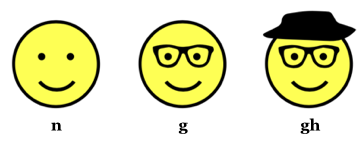
\includegraphics[width=.5\textwidth]{plots/faces-ad-hoc-implicature.png}
\caption{\label{fig:faces-ad-hoc-imp}: Referents in ad-hoc implicature reference game.}
\end{figure}

At the next level, pragmatic listeners $L_1$ try to infer the world state that the speaker intended to communicate
through Bayesian inference: $L_1$ integrates their prior beliefs about the state of the world $P(w)$ with the likelihood
of the speaker $S_1$ choosing the observed utterance to communicate $w$:
$$L_1(w \mid u) \propto P(w) \times S_1(u \mid w)$$

This recursive reasoning process can theoretically be continued ad infinitum by adding additional speaker and listener agents that 
reason about their respective counterpart agents one level below $i-1$ the current level $i$:
$$U_i(w,u) = \log L_{i}(w \mid u) - c(u)$$
$$S_i \propto \mbox{exp} \left( \lambda U_{i-1}(w,u) \right)$$
$$ L_i(u \mid w) \propto P(w) \times S_i(u \mid w)$$

\todo{mention IBR}

In practice, however, this recursive process is usually capped at the $L_1$ and $L_2$ level (\todo{add reference. Franke and Degen?}) and the models
that I will consider in this dissertation are also all capped at the $L_1$ level.



This recursive reasoning process implicitly models a Gricean counterfactual reasoning process in which listeners reason about alternative utterances
that a speaker could have produced but didn't to interrpret To illustrate how this works, consider a simple reference game as shown in Figure~\ref{fig:faces-ad-hoc-imp}.\footnote{Example adapted from \textcite{Goodman2016}.} In this game,
there are three faces: one without any accessories (\textbf{n}), one with glasses (\textbf{g}), and one with glasses and a hat (\textbf{gh}). A speaker chooses one of the three faces
and tries to communicate her choice to the listener through an utterance $u$. In this contrived example, let us assume that the only three possible utterances that the
speaker can choose from are $U=\{\mbox{\textsc{face}: My friend has a face},\mbox{\textsc{glasses}: My friend has glasses},$ $\mbox{\textsc{hat}: My friend has a hat}\}$, 
and that the listener is aware that the speaker can only choose from these three utterances. Speakers tend to show the following behavior in this game. If they refer
to \textbf{n}, they produce \textsc{face}, if they refer to \textbf{g}  they produce \textsc{glasses}, and if they refer to \textbf{gh} they produce \textsc{hat}. Conversely, listeners infer that 
the speaker likely referred to \textbf{n} after hearing \textsc{face}, to \textbf{g}  after hearing \textsc{glasses}, and to \textbf{gh} after hearing \textsc{hat}.

An RSA model rooted at a literal listener $L_0$ with a pragmatic speaker $S_1$ and a pragmatic listener $L_1$ captures this behavior. In this game, 
the semantic interpretation function $\sem{\cdot}$ is defined as:

\begin{center}
\begin{tabular}{c | c } 
$u$ & \sem{u} \\ \midrule
\textsc{face} & $\{\mathbf{n}, \mathbf{g} , \mathbf{gh}\}$  \\
\textsc{glasses} & $\{ \mathbf{g} , \mathbf{gh}\}$ \\
\textsc{hat} &$\{\mathbf{gh}\}$ \\
\end{tabular}
\end{center}

\noindent Computing the distributions for $L_0 (w\mid u)$ -- if we assume uniform priors over the three referents -- then results in:

\begin{center}
\begin{tabular}{c | c | c | c} 
$u$ & $L_0( \mathbf{n} \mid u)$ &  $L_0( \mathbf{g} \mid u)$ &  $L_0( \mathbf{gh} \mid u)$ \\ \midrule
\textsc{face} & $\frac{1}{3}$ & $\frac{1}{3}$ & $\frac{1}{3}$  \\
\textsc{glasses} &0  & $\frac{1}{2}$ & $\frac{1}{2}$  \\
\textsc{hat} & 0 & 0 & 1 \\
\end{tabular}
\end{center}

\noindent At the two extremes, $L_0$ thus chooses a face at random after hearing \textsc{face}, which is true about all three 
faces but it will always choose \textbf{gh} after hearing \textsc{hat}, which is only true for \textbf{gh}. As I mentioned above, the
pragmatic speaker $S_1$ then chooses an utterance by soft-maximizing their utility, which depends on the informativity of $u$
to communicate $w$ to $L_0$ and the cost $c(u)$, which I assume to be 0 for all utterances in this example. If we further assume
that the rationality parameter $\lambda=1$, then $S_1(u \mid w)$ is:

\begin{center}
\begin{tabular}{c | c | c | c} 
$w$ & $S_1( \textsc{face} \mid w)$ &  $S_1( \textsc{glasses} \mid w)$ &  $S_1( \textsc{hat} \mid w)$ \\ \midrule
\textbf{n} & 1  & 0 & 0  \\
\textbf{g} &$\frac{2}{5}$  & $\frac{3}{5}$ & 0  \\
\textbf{gh} & $\frac{2}{11}$ & $\frac{3}{11}$ & $\frac{6}{11}$ \\
\end{tabular}
\end{center}

\noindent This speaker model qualitatively predicts the behavioral data from forced choice production experiments \cite{Goodman2016}: for all three
referents the most likely utterance choice according to $S_1$ matches the most likely choice in the experimental data. However, this behavior could have
also been predicted by purely symbolic counterfactual reasoning processes as outlined in \textcite{Grice1975} and \textcite{Hirschberg1985}. The real advantage of this model 
comes from the fact that it is a quantitative model and if one fits the rationality parameter $\lambda$ to the experimental data, one can also quantitatively predict 
utterance choices in a population of participants.

Finally, the pragmatic listener $L_1(w \mid u)$ can be used to predict the interpretation of utterances in this context. If we again assume that the prior over referents $P(w)$
is uniform, $L_1$ is:

\begin{center}
\begin{tabular}{c | c | c | c} 
$u$ & $L_1( \mathbf{n} \mid u)$ &  $L_1( \mathbf{g} \mid u)$ &  $L_1( \mathbf{gh} \mid u)$ \\ \midrule
\textsc{face} & $\frac{55}{87}$ & $\frac{22}{87}$ & $\frac{10}{87}$  \\
\textsc{glasses} &0  & $\frac{11}{16}$ & $\frac{5}{16}$  \\
\textsc{hat} & 0 & 0 & 1 \\
\end{tabular}
\end{center}

\noindent This listener model qualitatively predicts the behavioral data from the interpretation experiments, and once again one can quantitatively predict participants' proportions
of choosing the three referents after hearing a given utterance by fitting the rationality parameter $\lambda$. 

Predicting utterance choices and interpretations in this contrived example of an ad-hoc implicature may not seem particularly impressive. However, many subsequent works
following the original RSA model have extended this basic model to predict a wide range of pragmatic phenomena, including predicting scalar inferences 
\cite{Goodman2013}, embedded implicatures \cite{Potts2016}, M-implicatures \cite{Bergen2016}, metaphors and hyperbole \cite{Kao2014a,Kao2014b}, 
irony \cite{Kao2015,CohnGordon2019}, the use of gradable adjectives \cite{Lassiter2017b, Qing2015}, generics \cite{Tessler2019}, vague quantifiers 
\cite{Scholler2017}, politeness \cite{Yoon2018}, social meaning \cite{Burnett2019}, and--as I will discuss in more detail in the next chapter--to 
predict the use and interpretations of epistemic modals \cite{Herbstritt2019}. While almost all of these models 
introduce additional extensions to the model as presented here, they crucially all rely on the recursive Bayesian reasoning process outlined in this section,
highlighting the versatility of models that cast pragmatic behavior as an instance of recursive Bayesian reasoning.





